\chapter{Background and Theory}

This chapter will provide information about hardware, software and different topics important for understanding the results. 

\section{Hardware}
The hardware used in this exercise is the EFM32GG-DK3750 development board from Silicon Labs depicted in Figure \ref{fig:devboard}. It was connected to a personal computer via USB. It also includes a TFT screen which can display real-time energy consumption. The EFM32GG uses the energy efficient 32-bit ARM Cortex-M3. It's worth mentioning that the M3 uses Harvard architecture \cite{cortexm3}, which allows it to read input at the same as it can execute instructions.

\subsection{Sound and DAC}
\label{sec:dac}
The board has an integrated DAC (digital-to-analog converter), which will be used for playing music and sound effects. A DAC takes input as digital data, a stream of binary values, and outputs analog values in the form of voltage or current.

Sound is best described mathematically as sine waves. These waves pushes the air at a given frequency. This frequency determines the pitch or tone. The human ear can hear sound with frequencies in the range from roughly 20Hz to 20kHz.

Since a DAC takes discrete values as input, you can generate an output that best resembles the sound by taking samples of the sine wave. The more samples you have per period, the higher the quality of the output.

\subsection{Timer and Clock}
\label{sec:timer}
The EFM32GG has a high frequency clock, HFRCLK, which is usually driven by the high-frequency oscillator HFRCO, but can also be driven by another high-frequency oscillator, or one of the low-frequency oscillator. The HFRCLK drives the prescalers that generate the high-frequency peripheral clock (HFPERCLK) and the high-frequency core clock (HFCORECLK). The HFRCLK can be divided down to run on a lower frequency, which then in turn will lower the HFPERCLK and HFCORECLK.

The EFM32GG also has 

20.3.1 Counter Modes START HERE NOW, AND DON'T WINE ABOUT BEING HUNG OVER.


\subsection{Gamepad}
In addition we had a gamepad with eight buttons and eight LEDs depicted in Figure \ref{fig:gamepad}. This was connected to the development board's GPIO pins. The gamepad includes a jumper, that when set to the lower two pins will exclude the LEDs form the power measurement. 

\begin{figure}
\centering
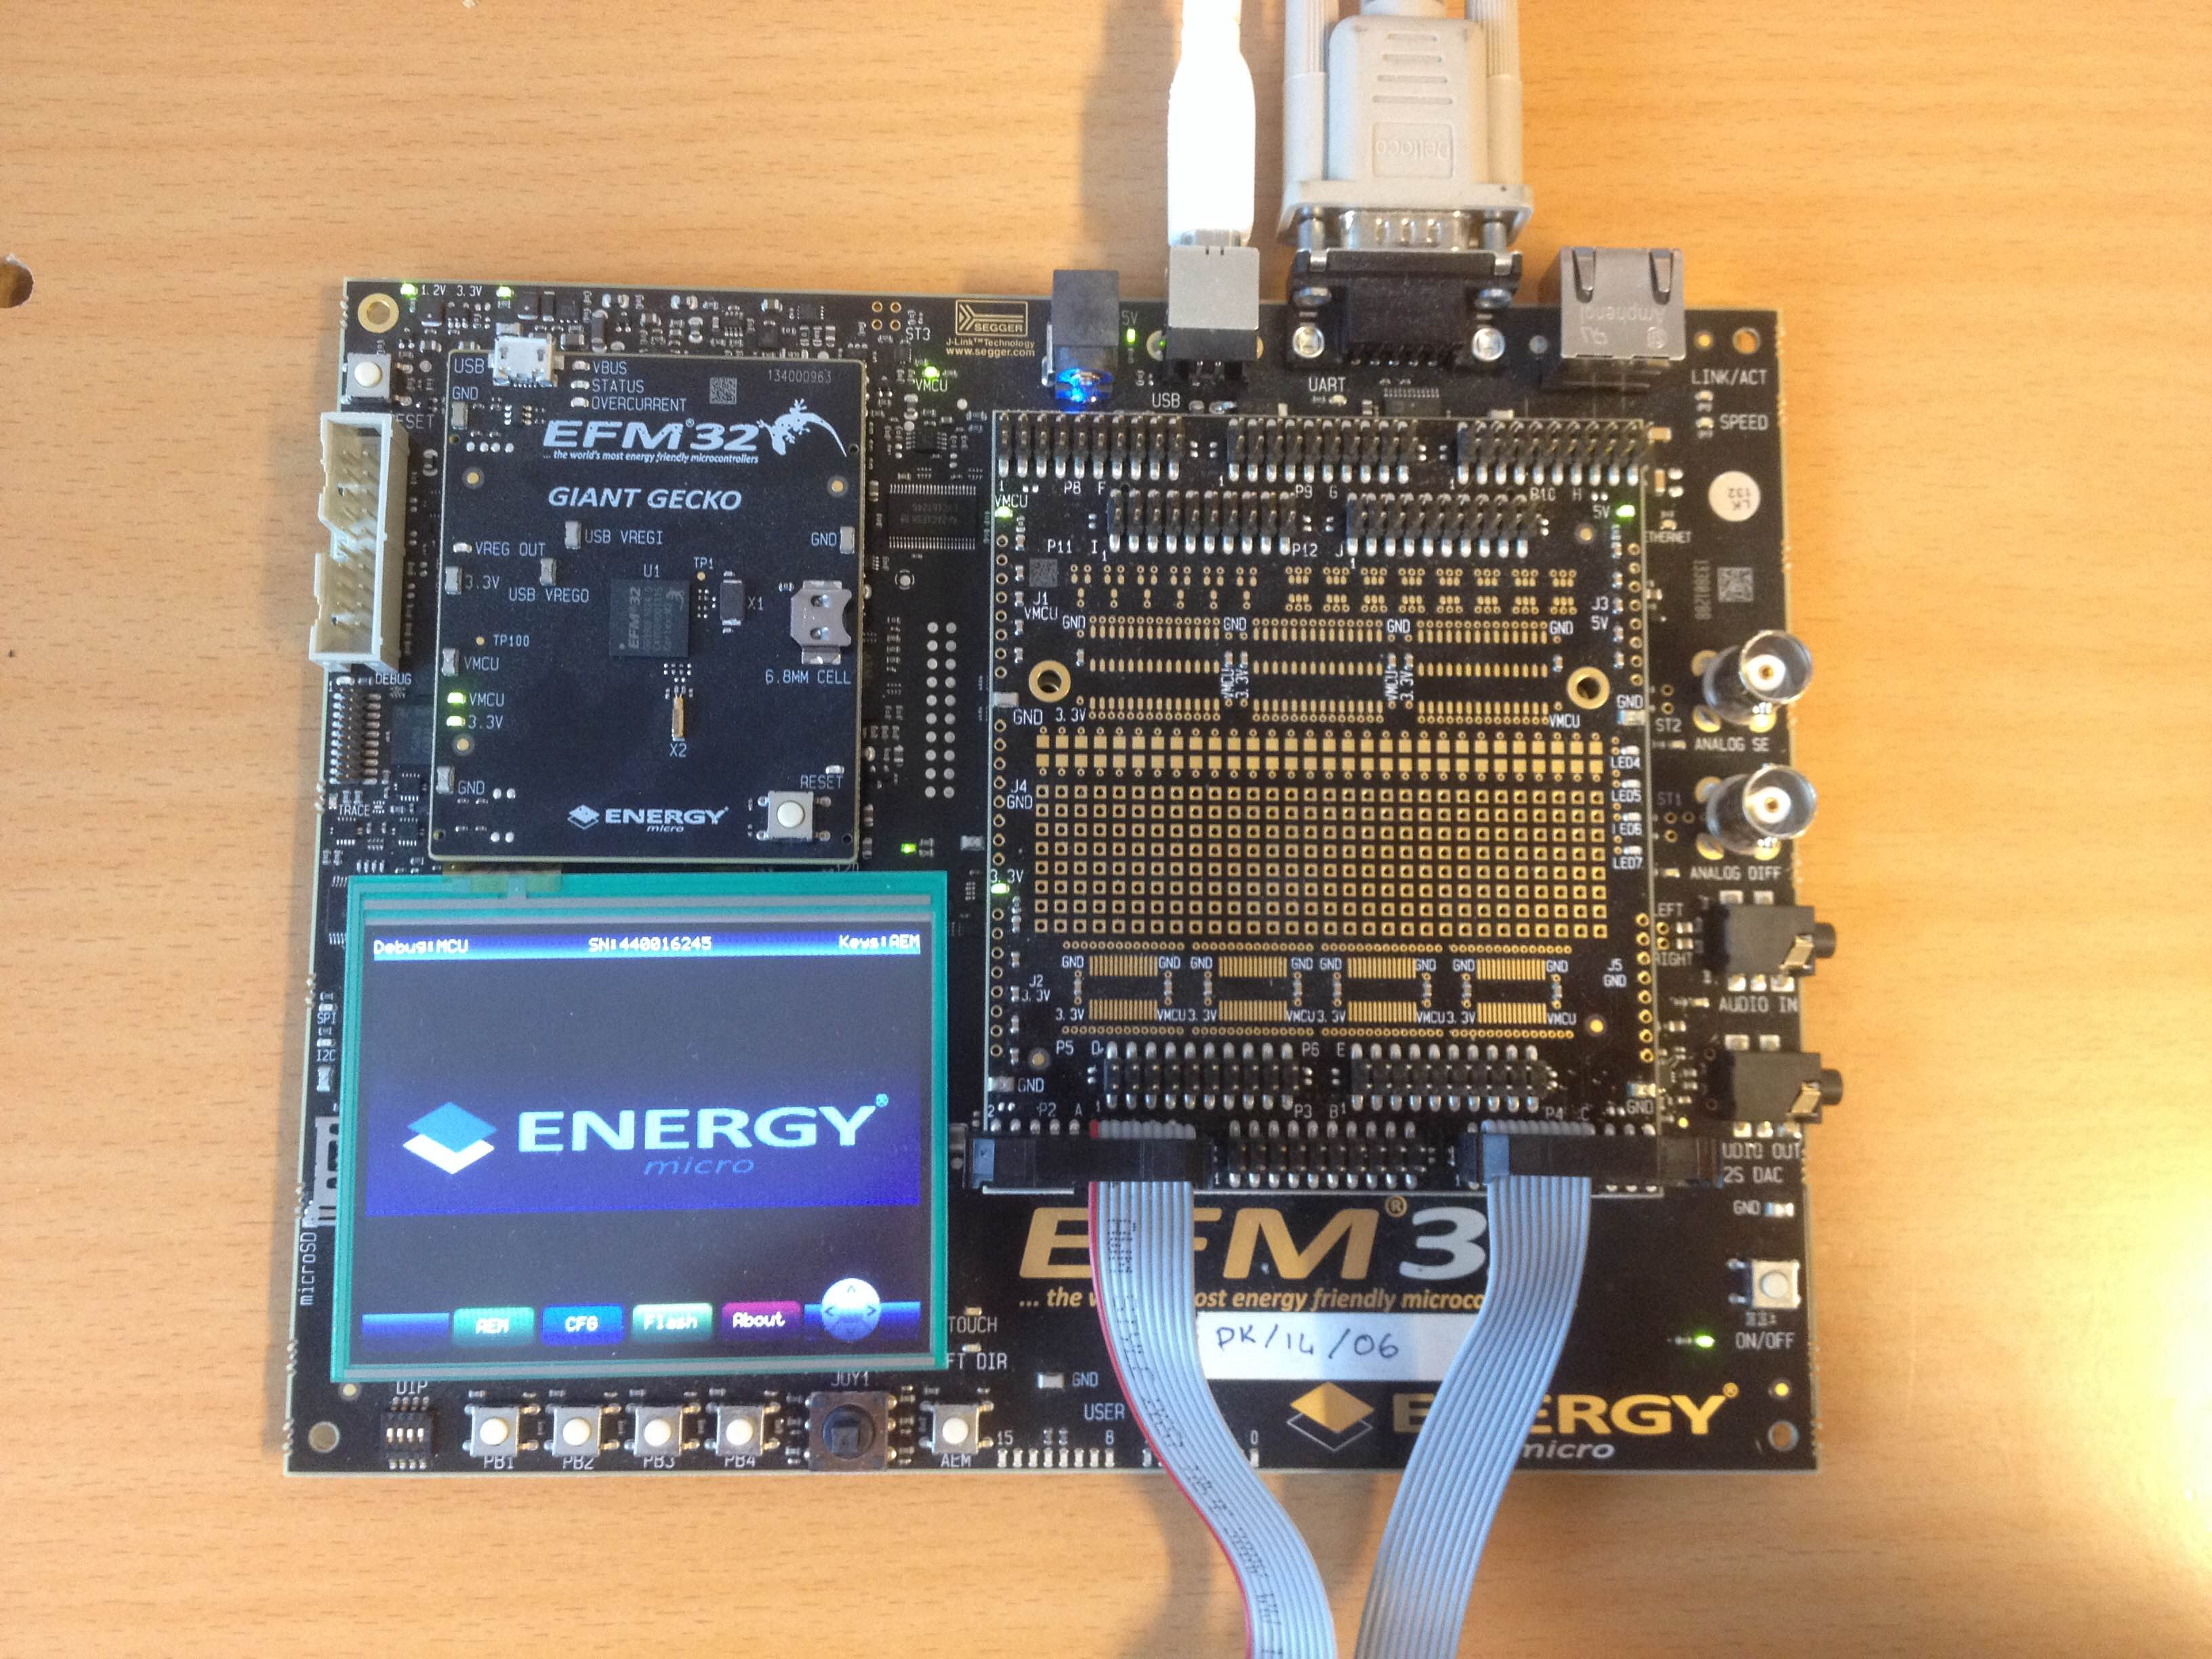
\includegraphics[scale=0.1]{images/EFM32GG-DK3750.jpg}
\caption{EFM32GG-DK3750}
\label{fig:devboard}
\end{figure}

\begin{figure}
\centering
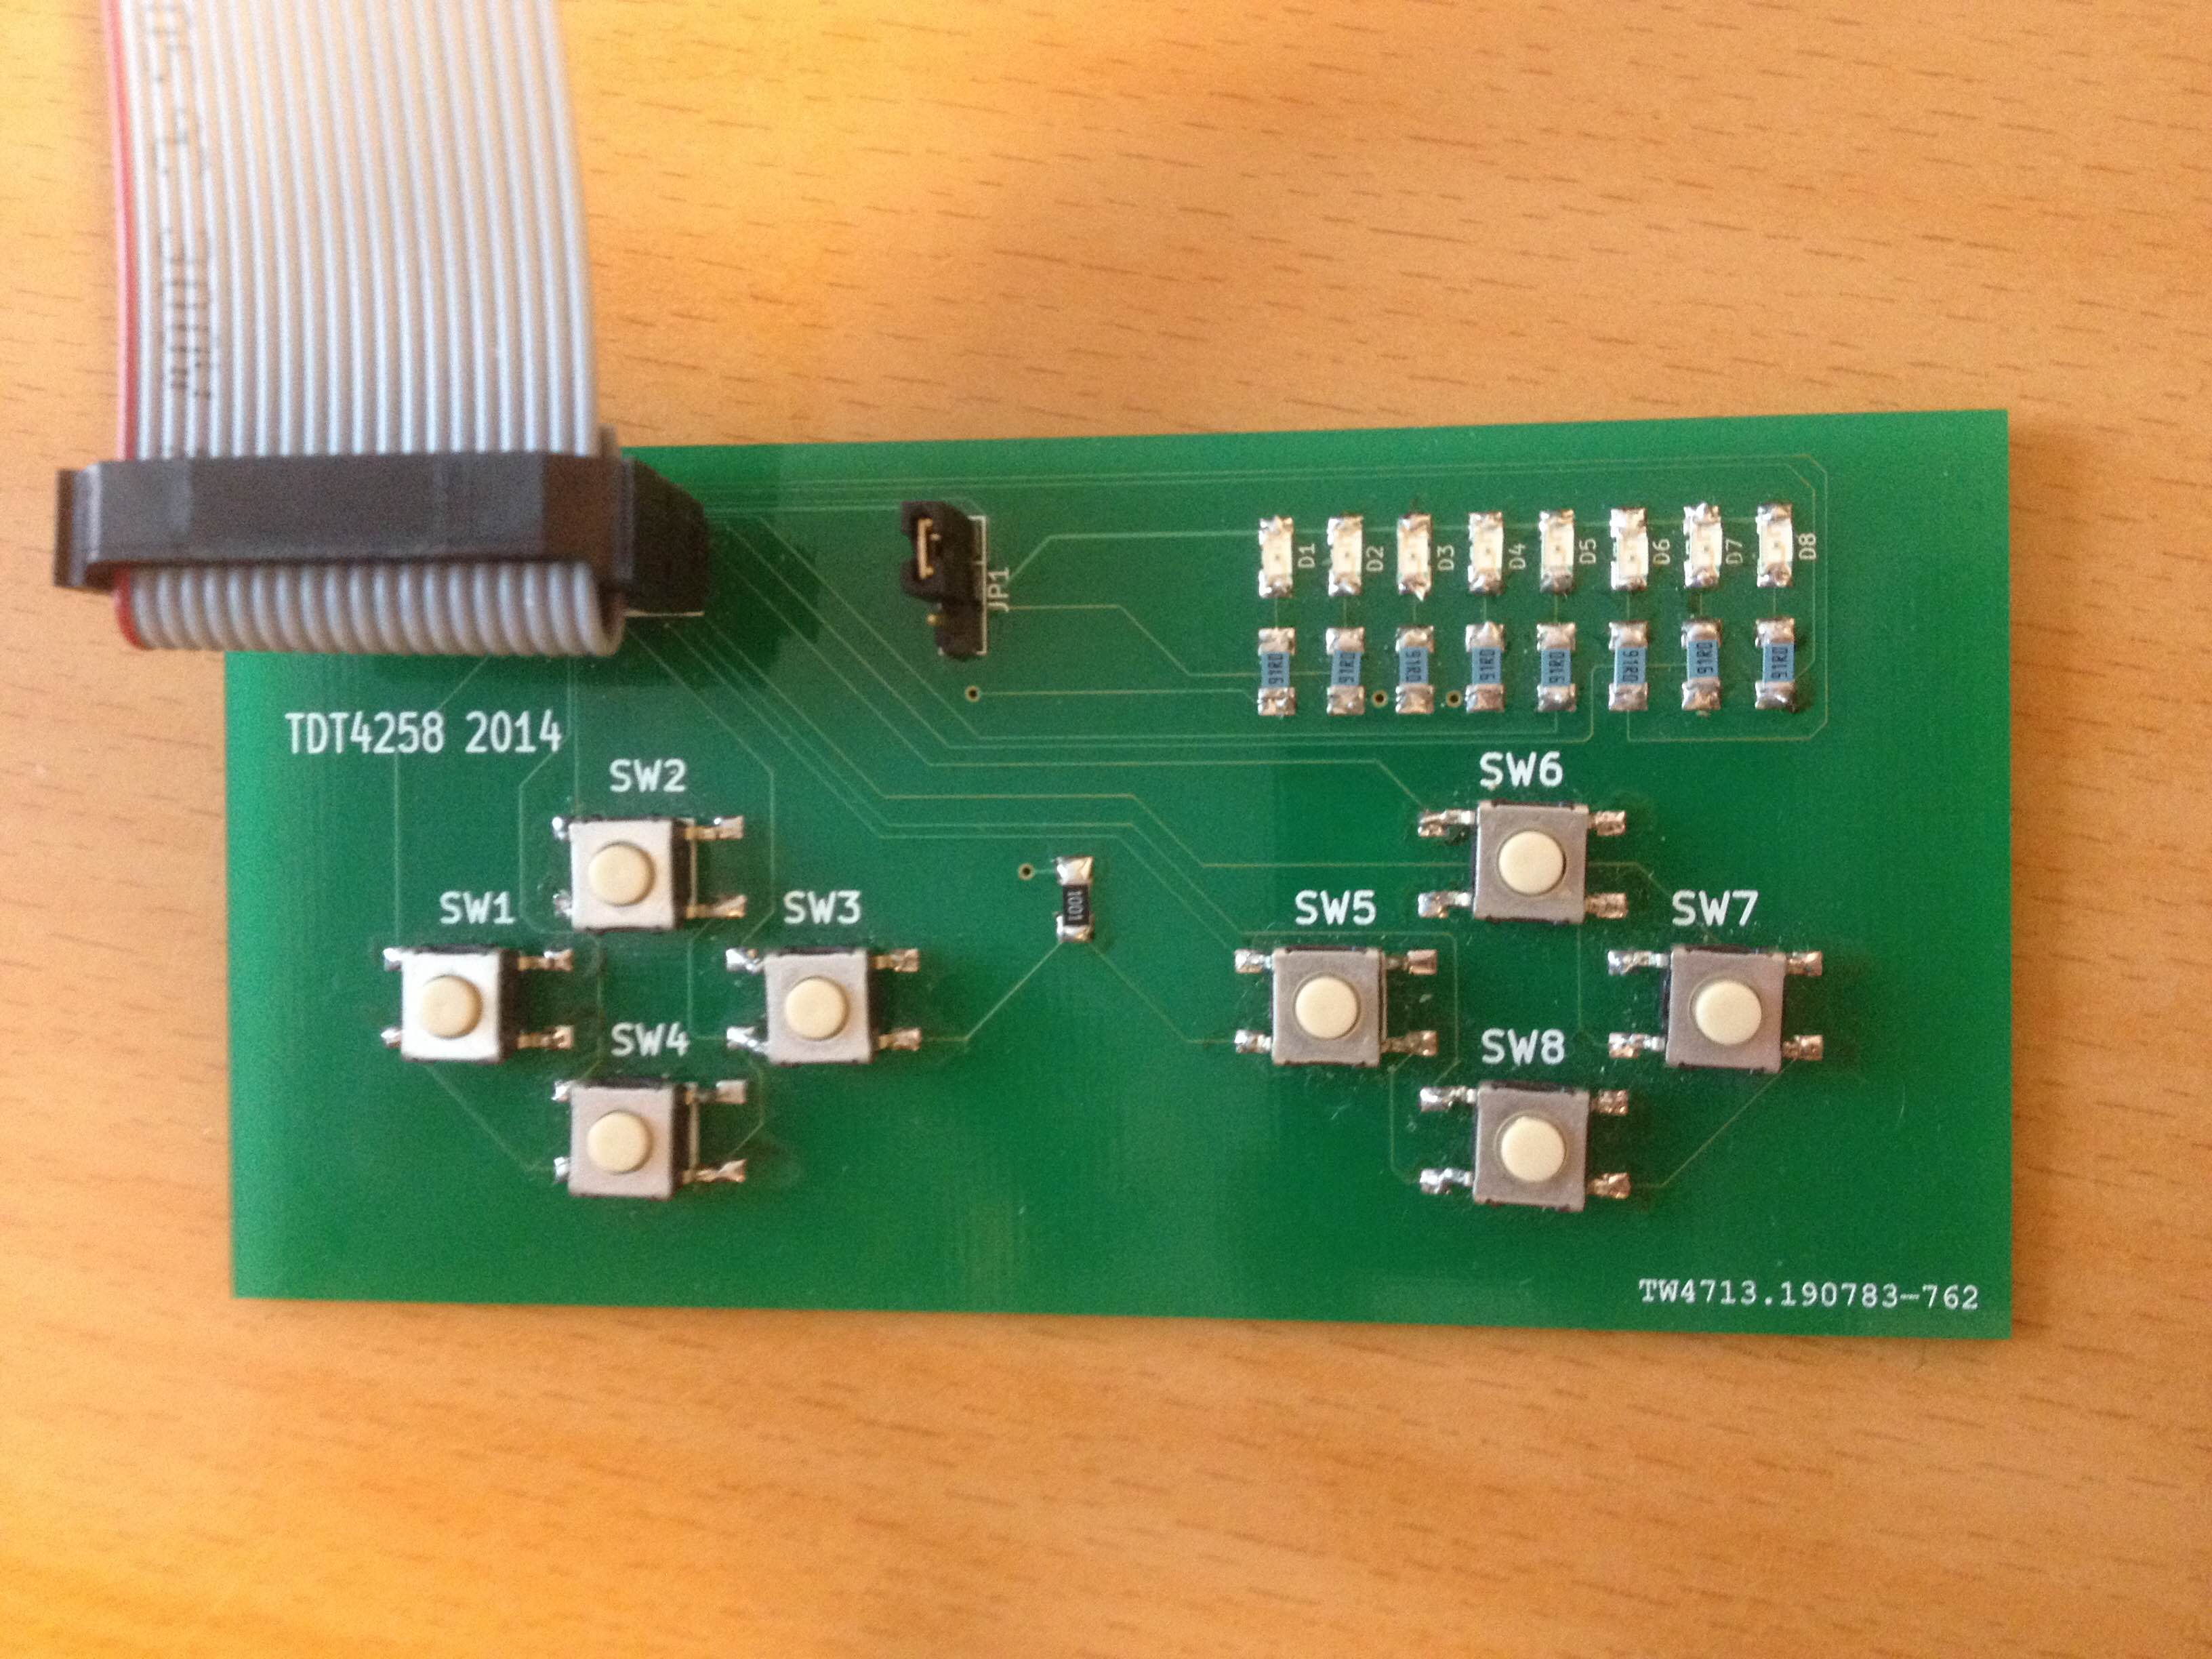
\includegraphics[scale=0.1]{images/gamepad.jpg}
\caption{Gamepad}
\label{fig:gamepad}
\end{figure}


\section{Static vs dynamic power consumption}
\label{sec:static}
The total power consumption is the sum of static- and dynamic power consumption, given by Formula 2.1, acquired from the course's lecture notes:

\begin{gather}
\label{cycle-formula}
P_{tot} = P_{dynamic} + P_{static} = \alpha C V^{2} f + I_{static} V
\end{gather}

There is static power consumption due to leakage in the transistors. The gate oxide layer in a transistor is not a perfect insulator, and therefore there will always be some current leaking through an active transistor. 

The dynamic power consumption comes from when a transistor changes state, i.e. goes from 0 to 1 or vice versa, and is dependant on the capacitance of the transistors. The thing worth mentioning is that the voltage is squared, and it is key to keep the voltage as small as possible.

The total energy consumption is given by:

\begin{gather}
\label{cycle-formula}
E = P_{total} t
\end{gather}

The static power consumption of a system is constant, but the dynamic consumption is dependant on the clock frequency. The time it takes for a certain amount of work to complete is dependent on the clock. Therefore, reducing the clock frequency will actually increase the total energy usage, because the program will need to run for a longer period. The static power consumption is present for a longer time, and as a result, it is often best to do the calculations without downscaling the clock, and then turn the components off.

\section{The C language}
C is a low-level, imperative programming language. It is a general purpose language, which also provides a lot of control for the programmer with regards to memory control and memory access. A very useful part of C is pointers. Pointers contain addresses to memory locations, and can be dereferenced to obtain the value on the given location. This is very useful when programming microcontrollers, because it makes it easy to write and obtain values directly from memory.

\section{Energy Efficiency}

There are a lot of ways of reducing the power needed to run programs, and the following section describes some of these techniques.

\subsection{Energy Modes on the EFM32GG}
The EFM32GG has five different energy modes, all with different levels of active components and power consumption. Figure \ref{fig:em} shows an overview of the EFM32GG and Figure \ref{fig:em2} shows a color scheme with the different energy modes indicated with a respective number. The colors in Figure \ref{fig:em} translates to the highest energy mode in which they are active.

Here are some of the key aspects worth noticing about each energy mode:

\begin{description}
  \item[EM0 - Run] Everything is active.
  \item[EM1 - Sleep] The CPU is sleeping, the rest is active.
  \item[EM2 - Deep Sleep] High frequency oscillators, flash memory, timer/counter are inactive
  \item[EM3 - Stop] RAM, DAC and external interrupts are still active.
  \item[EM4 - Shutoff] Everything is shut off, only a reset can turn it on again.
\end{description}

\begin{figure}[h]
\centering
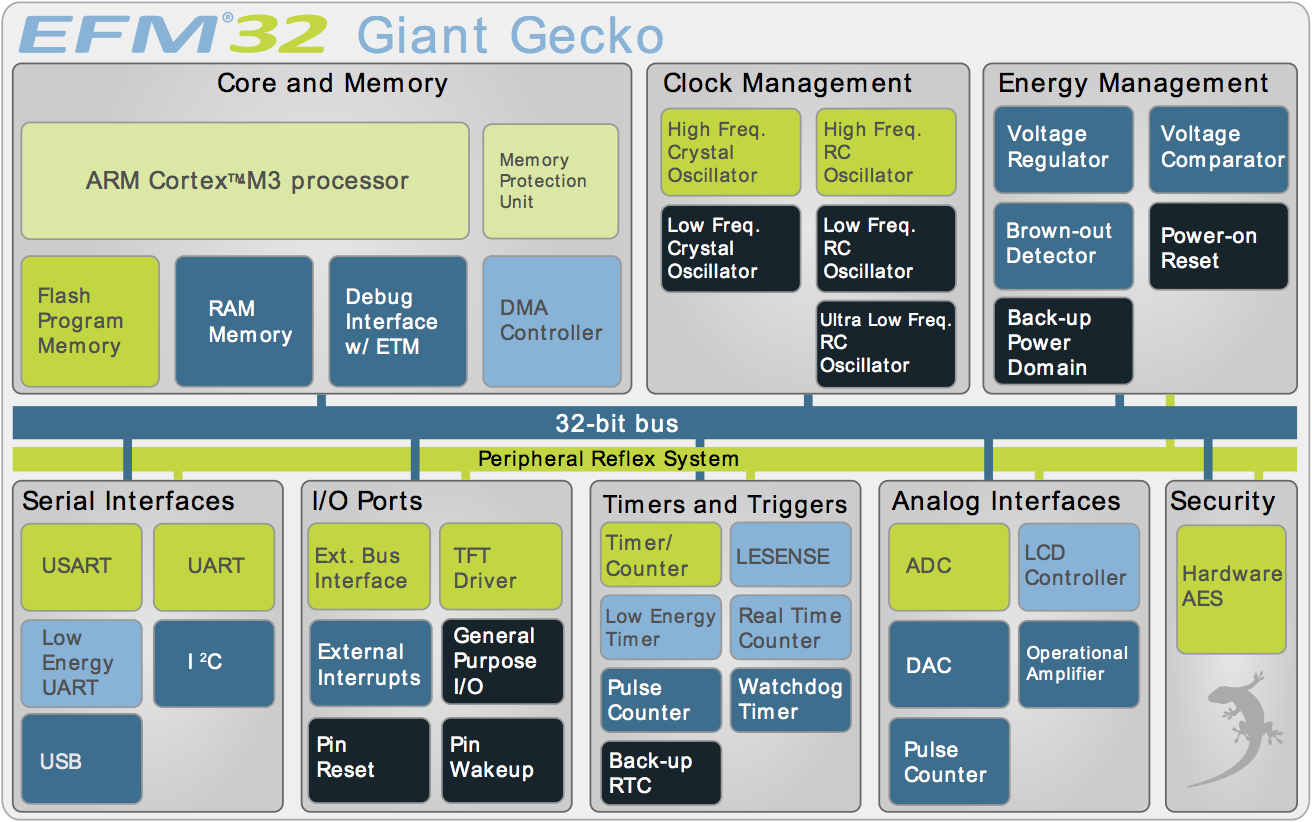
\includegraphics[scale=0.6]{images/em.png}
\caption{Diagram of EFM32GG}
\label{fig:em}
\end{figure}

\begin{figure}[h]
\centering
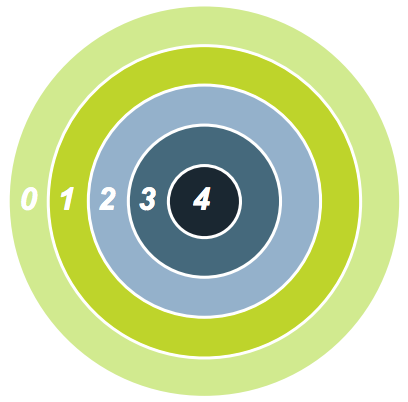
\includegraphics[scale=0.6]{images/em_numbers.png}
\caption{Energy Mode Indicator}
\label{fig:em2}
\end{figure}

\subsection{Interrupts}
\label{sec:interrupts}
When a program is idle, there are several ways to wake it up. One way is by using polling. Polling is when you repeatedly check the status of a unit to see if there are any changes or if it is ready for use. This is not very efficient with regards to energy efficiency, because you continuously check to see if there is work to be done, and you use a lot of processing power. 

A good replacement for polling is the use of interrupts. An interrupt is a signal to the processor indicating that an event needs immediate attention. When the processor receives an interrupt signal, it suspends its current program and executes a handler routine defined in the interrupt handler vector. After the handler routine is completed, the processor returns to the program it was originally executing\cite{wolf2012computers}. The use of interrupts will relieve the processor of a lot of work, and only do work when it's needed, which in turn decreases the energy consumption.

\subsection{Reducing Static Power Consumption}
As described in Section \ref{sec:static}, there is always static power consumption when a transistor is active. One way of reducing the total energy consumption, is by simply turning off parts of the system that are not in use, and thus decreasing the total static power consumption. 